%%%%%%%%%%%%%%%%%%%%%%%%%%%%%%%%%%%%%%%%%
% Large Colored Title Article
% LaTeX Template
% Version 1.1 (25/11/12)
%
% This template has been downloaded from:
% http://www.LaTeXTemplates.com
%
% Original author:
% Frits Wenneker (http://www.howtotex.com)
%
% Modified for use in class at Olin College of Engineering
%
% License:
% CC BY-NC-SA 3.0 (http://creativecommons.org/licenses/by-nc-sa/3.0/)
%
%%%%%%%%%%%%%%%%%%%%%%%%%%%%%%%%%%%%%%%%%

%----------------------------------------------------------------------------------------
%	PACKAGES AND OTHER DOCUMENT CONFIGURATIONS
%----------------------------------------------------------------------------------------

\documentclass[11pt, twocolumn]{article}

\usepackage[english]{babel} % English language/hyphenation
\usepackage{graphicx}
\usepackage[usenames,dvipsnames,svgnames,table]{xcolor} %usenames: 16 HTML base colors%dvipsnames: 64 more colors%svgnames: 150 colors%table: colors in tables

\usepackage[hyphens]{url} 	%allow url references in bibtex
\usepackage[colorlinks=true,urlcolor=DarkRed,linkcolor=DarkRed,citecolor=DarkRed]{hyperref}
%\renewcommand{\href}[2]{\href{#1}{\url{#2}}}
%\href{mailto:jomm@olin.edu}{jomm at olin dot edu}

\overfullrule=2cm%show overfull locations; useful for debugging

\usepackage[fleqn]{amsmath} % Math packages
\interdisplaylinepenalty=2500 %don't allow line breaks in the middle of multi-line equations

\usepackage[margin=1in]{geometry}
\linespread{1.03}
%\usepackage{parskip}%add spacing between paragraphs
\setlength{\parindent}{20pt}%15pt normally

\usepackage[hang, normal,labelfont=bf,up,textfont=it,up]{caption} % Custom captions under/above floats in tables or figures
\usepackage{booktabs} % Horizontal rules in tables

\usepackage{sectsty} % Enables custom section titles
\allsectionsfont{\usefont{OT1}{phv}{b}{n}} % Change the font of all section commands

\usepackage{fancyhdr} % Needed to define custom headers/footers
\pagestyle{fancy} % Enables the custom headers/footers
\usepackage{lastpage} % Used to determine the number of pages in the document (for "Page X of Total")

% Headers - all currently empty
\lhead{}
\chead{}
\rhead{}

% Footers
\lfoot{\footnotesize \today}
\cfoot{}
\rfoot{\footnotesize Page \thepage\ of \pageref{LastPage}} % "Page 1 of 2"

\renewcommand{\headrulewidth}{0.0pt} % No header rule
\renewcommand{\footrulewidth}{0.4pt} % Thin footer rule


%----------------------------------------------------------------------------------------
%	TITLE SECTION
%----------------------------------------------------------------------------------------

\usepackage{titling} % Allows custom title configuration

\newcommand{\HorRule}{\color{DarkGoldenrod} \rule{\linewidth}{1pt}} % Defines the gold horizontal rule around the title

\pretitle{\vspace{-30pt} \begin{flushleft} \HorRule \fontsize{50}{50} \usefont{OT1}{phv}{b}{n} \color{DarkRed} \selectfont} % Horizontal rule before the title

\title{Rad Title} % Your article title

\posttitle{\par\end{flushleft}\vskip 0.5em} % Whitespace under the title

\preauthor{\begin{flushleft}\large \lineskip 0.5em \usefont{OT1}{phv}{b}{sl} \color{DarkRed}} % Author font configuration

\author{Rad Student, } % Your name

\postauthor{\footnotesize \usefont{OT1}{phv}{m}{sl} \color{Black} % Configuration for the institution name
Olin College of Engineering % Your institution

\par\end{flushleft}\HorRule} % Horizontal rule after the title

%----------------------------------------------------------------------------------------
\date{} % Add a date here if you would like one to appear underneath the title block

\begin{document}

\maketitle % Print the title

\thispagestyle{fancy} % Enabling the custom headers/footers for the first page 

%----------------------------------------------------------------------------------------
%	ABSTRACT
%----------------------------------------------------------------------------------------

% The first character should be within \initial{} for a large character
\noindent \textbf{This is the abstract text. It should summarize the main idea of the paper. Don't write abstracts that say ``I will analyze x and focus on y''. This is akin to saying ``In this paper, I will introduce a subject as mentioned in my title, analyze data relevant to it, and discuss some conclusions.'' The abstract is the juiciest possible content.}

%----------------------------------------------------------------------------------------
%	ARTICLE CONTENTS
%----------------------------------------------------------------------------------------

\section*{Phase I feedback}
Include everything in your folder: the paper and the latex source, the graphics, python programs, excel sheets and data files (unless they're huge and easily accessible, in which case provide a link to the source) and references. Basically, anyone should be able to continue your work by downloading your folder.

Make you graphics big! In order to let a figure extend the two columns, add an asterisk (*) after figure like this:
\begin{verbatim*}
\begin{figure*}
...
\end{figure*}
\end{verbatim*}



Careful with passive voice. Avoid it, or make sure you know who does the action.

Don't tell the reader how to feel or judge a fact. Avoid: ``This is important because...'' Just state the fact or relationship, and let the reader judge. I imagine a reader that does not want to believe me and write statements that are undeniable given the data and facts.

Make sure you spell out an acronym the first time you use it and put it in parenthesis right after.

Make sure you clearly indicate where you found every dataset and image with a specific webpage or link (sites are huge). Better to be repetitive than not.

Caption should be more than titles. Anyone reading just the captions should get a sense of the whole story.

Figures and tables should always be referenced within the text, as in the case of Figures~\ref{fig:myfigure} and~\ref{fig:myfigure2} and Table~\ref{tab:mytable}.

\begin{figure*}
\centering 
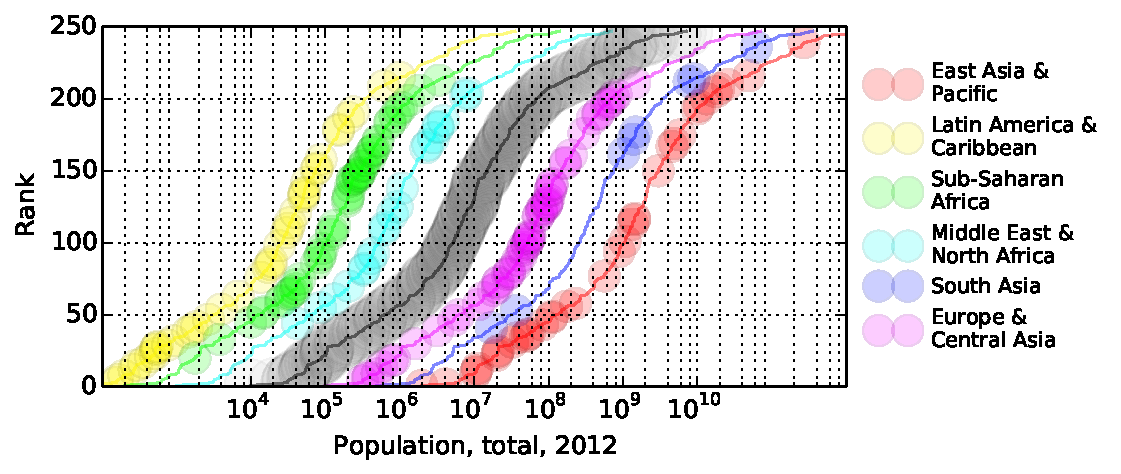
\includegraphics[width=\textwidth]{Populati2012.pdf}\caption{\label{fig:myfigure}As much as possible, the graph should speak by itself. However, you should write a caption that captures a more nuanced analysis of the dataset. The source citation should be in the caption directly. {\tt Data: World Bank World Development Indicators~\cite{wdi}. Source code for figure:~\href{https://github.com/jabb1123/RADical/blob/master/Oscar/wdiplot_population.py}{wdiplot\_population.py}.}} 
\end{figure*}

\begin{figure*}
\centering 
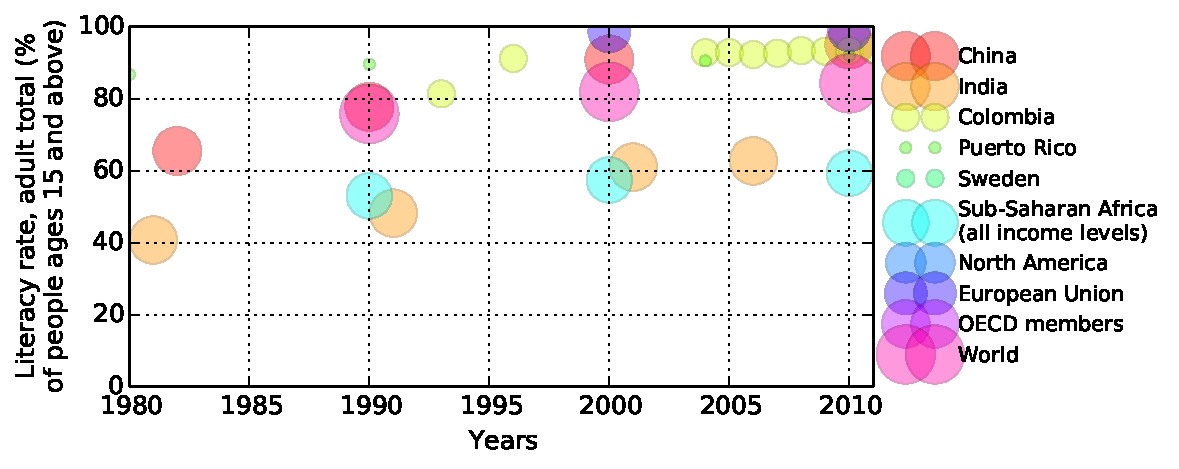
\includegraphics[width=\textwidth]{Literacy.pdf}\caption{\label{fig:myfigure2}As much as possible, the graph should speak by itself. However, you should write a caption that captures a more nuanced analysis of the dataset. The source citation should be in the caption directly. {\tt Data: World Bank World Development Indicators~\cite{wdi}. Source code for figure:~\href{https://github.com/jabb1123/RADical/blob/master/Oscar/wdiplots.py}{wdiplots.py}.}}
\end{figure*}

\section*{Testing Citations}
Citing papers~\cite{cnn},~\cite{prb} and~\cite{ssrc}.


\begin{table}
\caption{\label{tab:mytable}Random table}
\centering
\begin{tabular}{llr}
\toprule
\multicolumn{2}{c}{Name} \\
\cmidrule(r){1-2}
First name & Last Name & Income \\
\midrule
John & Doe & $\$15,000$ \\
Richard & Miles & $\$45,000$ \\
\bottomrule
\end{tabular}
\end{table}

References should be done like this~\cite{collier2001}.

\subsection*{Subsection 1}

The align environment is ideal to include math:
\begin{align}
A = 
\begin{bmatrix}
A_{11} & A_{21} \\
A_{21} & A_{22}
\end{bmatrix}
\end{align}

Itemized list:
\begin{itemize}
\item First item in a list 
\item Second item in a list 
\item Third item in a list
\end{itemize}

Dictionary list example:
\begin{description}
\item[First] This is the first item
\item[Last] This is the last item
\end{description}


%----------------------------------------------------------------------------------------
%	REFERENCE LIST
%----------------------------------------------------------------------------------------

\begin{thebibliography}{9}

\bibitem{collier2001}
Collier, Paul and Dollar, David, (2001), Can the World Cut Poverty in Half? How Policy Reform and Effective Aid Can Meet International Development Goals, World Development, 29, issue 11, p. 1787-1802.

\bibitem{wdi}
World Bank. World Development Indicators (WDI) online database. Washington, DC. \url{http://data.worldbank.org/data-catalog/world-development-indicators}. Data retrieved September 24, 2014.

\bibitem{cnn}
Davies, Catriona. ``Mideast Women Beat Men in Education, Lose out at Work." CNN. Cable News Network, 01 Jan. 1970. Web. 04 Dec. 2014. \url{http://www.cnn.com/2012/06/01/world/meast/middle-east-women-education/}.

\bibitem{prb}
Moghadam, Valentine M., and Farzaneh Roudi-Fahimi. ``Empowering Women, Developing Society: Female Education in the Middle East and North Africa." Population Reference Bureau, n.d. Web. 03 Dec. 2014. \href{http://www.prb.org/Publications/Reports/2003/EmpoweringWomenDevelopingSocietyFemaleEducationintheMiddleEastandNorthAfrica.aspx}{\tt{http://www.prb.org/Publications/Repor ts/2003/EmpoweringWomenDevelopingSoci etyFemaleEducationintheMiddleEastandN orthAfrica.aspx}}.
%\url{http://www.prb.org/Publications/Reports/2003/EmpoweringWomenDevelopingSocietyFemaleEducationintheMiddleEastandNorthAfrica.aspx}.

\bibitem{ssrc}
Shami, Seteney. ``Higher Education and Social Inequality in Comparative Perspective (U.S. and Egypt)." Social Science Research Committee, n.d. Web. 04 Dec. 2014. \url{http://www.ssrc.org/programs/higher-education-and-social-inequality-in-comparative-perspective-us-and-egypt/}.

\end{thebibliography}

%----------------------------------------------------------------------------------------

\end{document}